\section{Détail de la partie web du projet}
\par
Cette partie aura pour but de présenter la partie Web du projet sous un oeil technique. On présentera donc en détail les méthodes utilisées ainsi que les choix techniques qui composent notre projet.
	\subsection{La base de données}
	\par
	La base de données, qui est une base MySQL comme dit précédemment, se compose de 3 tables. De base, nous avions opté pour 2 tables : l'une pour stocker les utilisateurs de la plateforme et leur mot de passe relatif, l'autre pour stocker les capteurs et la mise à jour des données.
	\par
	Ce modèle était valide pour nos tests de début de projet mais s'est montré très limité quand nous avons décidé d'analyser les données des capteurs et spécialement quand nous avons décidé de stocker dans la durée les données. Par exemple, nous avions besoin de plusieurs données d'un même capteur pour dessiner un graphe ou plus simplement comparer différentes mesures.
	Comme nous stockions uniquement la dernière mesure (les informations étaient écrasées à chaque mise à jour), nous ne pouvions stocker plusieurs mesures d'un même capteur. Nous avons donc changé notre implémentation des tables dans la base.
	\par
	Nous aurions pu garder seulement 2 tables, en insérant simplement les nouvelles données dans la table des capteurs au lieu de mettre à jour les champs correspondant. Cette idée n'a pas pu être mise en place car cette table possède un champ 'ID' qui est la clé primaire de la table. Or il aurait fallu avoir plusieurs entrées comportant le même 'ID', ce qui est impossible.
	\par
	C'est donc à ce moment là que la table des capteurs est devenue la table répertoriant la liste des capteurs et une nouvelle table stockant toutes les données des capteurs a été crée.
	\par
	Les relations entre ces différentes tables sont schématisées sur la figure suivante et détaillées ci dessous:
	 \begin{figure}[h]
  		\centering
    		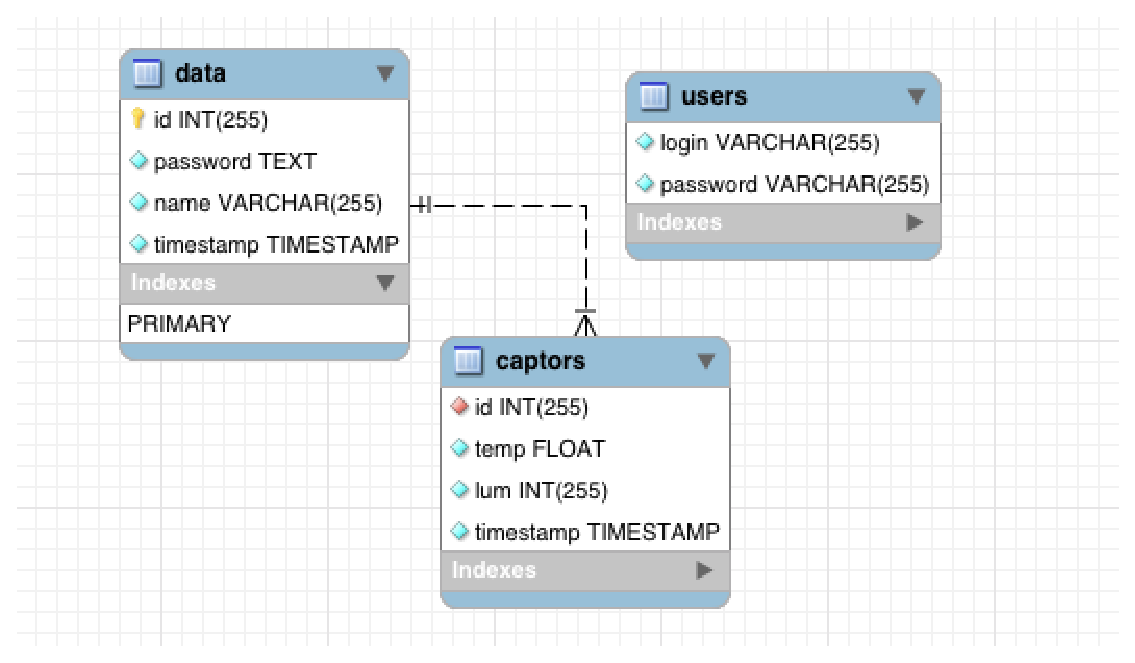
\includegraphics[scale=0.5]{diagramme_tables.eps}
		\caption {diagramme des tables}
	\end{figure}
	\par
	La table 'users' répertorie les différents utilisateurs de la plateforme Web. C'est à travers elle qu'un utilisateur est autorisé à se connecter, sous réserve que son nom et son mot de passe sont corrects.
	\par
	La table 'data' est la table répertoriant les différents capteurs. C'est à travers elle qu'un capteur est autorisé à mettre à jour ses données. Elle stocke aussi la date de dernière mise à jour du de chaque capteur.
	\par
	La table 'captors' est la table stockant les données de chaque capteur. C'est en quelque sorte l'extension de la table 'data'. Chaque champ, défini par son 'ID' ou son 'Name' est relié à une entrée de la table 'data' et complète cette dernière.
	\subsection{La plateforme}
	\par
	Le site se découpe en 4 modules (3 pour un utilisateur lambda) dont un visuel se situe en annexe.
	Pour construire ce site, nous avons utilisé différents langages et outils qui seront développés ci dessous.
	\subsubsection{Les différents modules}
	\par
	Le site Web contient 4 modules différents qui ont chacun une fonction particulière. Le premier est celui qui apparait en premier sur le site. Il autorise la connection à la plateforme. Une fois l'utilisateur connecté, il affiche les 5 dernières mises à jour des capteurs.
	\par
	Le deuxième module permet la recherche d'informations sur un capteur. La recherche s'effectue soit par 'ID' soit par 'Nom'. Une fois le capteur choisi, toutes les données disponibles le concernant s'affiche ansi que deux graphiques des 10 dernières mesures (un pour la température et un pour la luminosité).
	\par
	Le troisième module regroupe l'ajout et la suppression des capteurs. Il est nécessaire de déclarer et autoriser les capteurs en vue de leur mise à jour car si les capteurs ne sont pas répertoriés dans la base, leurs informations ne seront pas prise en compte (permet de sécuriser la mise à jour d'informations au cas où un tierce voudrait compromettre la base de données). Si le capteur n'est plus utilisé, on le supprime de la base à travers cette interface.
	\par
	Le dernier module n'est accessible qu'à l'administrateur de la plateforme. Il regroupe les fonctions d'administration : il permet l'ajout ou la suppression d'un utilisateur, la suppression complète des données des capteurs (en vue d'une remise à zéro) et un panneau de supervision. Ce dernier permet de repérer quels capteurs n'ont pas effectué leur mise à jour (en prenant comme référence la dernière heure). 
	\subsubsection{Le design : Ink}
	\par
	Pour cette plateforme, nous avons voulu faire quelque chose de visuellement propre. C'est donc dans cette optique que nous avons décidé d'utiliser un framework css. Ink est le framework libre qui s'occupe du design de notre site. Il nous a permis de donner un style simple à notre site, une fois maitrisé.
	\par
	La principale difficulté a été de comprendre comment fonctionnait Ink. En effet, en dehors des classes qui lui sont propres, il utilise un système de grille. Chaque morceau du site est découpé et se positionne sur la grille. Ce système structure le site et offre une interface épuré avec de nombreuses possibilité déjà implanté.
	\par
	L'utilisation de Ink se justifie par la qualité visuelle que l'on n'aurait pas pu atteindre par nous même, par manque de temps et certainement de talent graphique.
	\subsubsection{La gestion des données : PHP et Requêtes}
	\par
	L'interaction entre l'utilisateur et le base de données est assurée par PHP. C'est lui qui s'occupe de récupérer, mettre à jour et supprimer les informations demandées ou envoyées par l'utilisateur et le capteur. Il permet aussi d'executer du code en fonction de différents paramètres. C'est lui qui va être le moteur de l'application.
	\par
	Dans un premier temps, il permet d'executer et d'afficher sur la page ce qui est demandé par l'utilisateur, par exemple si l'utilisateur n'a pas encore demandé d'informations sur un capteur, on lui propose de faire un choix entre différents capteurs. Une fois qu'il en a sélectionné un (c'est à dire après l'envoi en POST du choix), PHP récupère cette information et prépare la page pour répondre à la demande de l'utilisateur. Pour illustrer cette fonction, on prend pour exemple le code suivant :
	\\%
	\lstset{language=PHP} 
	\begin{lstlisting}[frame=single]
/*Si on a recu une information d'ID, c'est a dire que l'utilisateur
demande une info sur une ID*/		
if(isset($_POST['id'])){
	//On execute les actions appropriees
}
	\end{lstlisting}
	\par
	La deuxième utilité de PHP est de pouvoir interagir directement avec la BDD. En utilisant PDO, on va se connecter à la base et executer des requêtes qu'on récupérera avec PHP.
	PDO est une méthode orientée objet d'interaction avec différents types de BDD (Mysql, PosgreSQL, etc...) qui est destiné à être la méthode principale à utiliser dans les prochaines versions de PHP. Le choix de PDO se justifie par sa capacité à préparer les requêtes avant de les executer  (on execute les requêtes en fonction de paramètres et non plus statiquement) et par l'importance qu'il prendra dans les versions futures de PHP (il est voué à être la méthode principale de connection, ce qui assure que l'application fonctionnera avec les versions futures).
	\par
	PDO fonctionne de la manière suivante :
	\\%
	\lstset{language=PHP} 
	\begin{lstlisting}[frame=single]
/*On instancie une variable PDO en PHP contenant
toutes les informations de connexion a la base de donnees*/
$bdd = new PDO('mysql:host=hostofthedatabase;dbname=nameofthedb', 
'user', 'password');
/*On prepare la requete avec en option un parametre
represente par "?"*/
$check=$bdd->prepare("SELECT login, password FROM users WHERE
login=?");
/*On execute la requete avec comme parametre "Jesuisunutilisateur"*/
$check->execute(array(Jesuisunutilisateur));
/*On recupere le resultat de la requete dans une variable pour une
utilisation ulterieure*/
$data=$check->fetch();
/*Une fois fini, on ferme proprement la connection a la base de 
donnees*/
$check->closeCursor();
	\end{lstlisting}
		
	\par
	Afin de gérer correctement les échanges d'informations entre le site et la base de données, quatre opérations différentes sont utilisées par PHP/PDO en utilisant le format MySQL :
	\\%
	\begin{itemize}
	\item Insérer des données dans la BDD : 
	\lstset{language=SQL} 
	\begin{lstlisting}[frame=single]
 Ex: INSERT INTO captors(temp,lum,timestamp,id) VALUES(?,?,?,?)
	\end{lstlisting}
	\item Obtenir des données de la BDD : 
	\lstset{language=SQL} 
	\begin{lstlisting}[frame=single]
Ex : SELECT login, password FROM users
	\end{lstlisting}
	\item Mettre à jour des données dans la BDD : 
	\lstset{language=SQL} 
	\begin{lstlisting}[frame=single]
Ex : UPDATE data SET timestamp=? WHERE id=?
	\end{lstlisting}
	\item Supprimer des données dans la BDD : 
	\begin{lstlisting}[frame=single]
Ex : DELETE  captors FROM captors WHERE timestamp  <  ?
	\end{lstlisting}
	\end{itemize}
	\subsubsection{Recup.php}
	\par
	La plus grosse partie du site consiste à faire interagir l'utilisateur avec la base de données. Cependant, il existe une page de site (recup.php) qui n'interagit pas avec l'utilisateur mais avec les capteurs. Celle ci reçoit des informations des capteurs (via POST), vérifie si le capteur a le droit de mettre à jour les données et effectue l'insertion dans la base.
	\par
	Cette page n'a pas seulement l'utilité de mise à jour, elle s'occupe aussi de la conversion des données de température. On s'est aperçu que les mesures brutes des capteurs n'était pas pertinentes et qu'il fallait multiplier les valeurs par 0,647 pour obtenir une valeur correcte.
	\par
	En dernier lieu, cette page se charge de nettoyer la table de données des capteurs en supprimer toute entrée datant de la veille via la fonction \href{http://www.php.net/manual/fr/function.date.php}{Date de PHP.}
	\subsubsection{Du dynamisme : Javascript} 
	\par
	Le Javascript sur le site est utilisé pour donner dynamiser l'utilisation du site. Il nous a permis de rediriger automatiquement l'utilisateur et principalement de gérer l'ajout de champ dans les pages d'ajout et de suppression de capteurs.
	En effet, nous l'avons utilisé pour permettre d'effectuer plusieurs actions identiques en une seule fois.
	\par
	Par exemple, quand on veut ajouter en chaine plusieurs capteurs, on aurait pu les ajouter un par mais cela aurait alourdi grandement l'application. La solution est simple, à chaque clic sur un bouton (dans notre cas, un "+"), le javascript insère un nouveau champ sur la page. 
	Cela se traduit par le code suivant : 
	\\%
	\lstset{language=Java} 
	\begin{lstlisting}[frame=single]
// On recupere le cadre ou on va inserer le nouvel element
var div = document.getElementById('champs');

// Fonction qui va creer l'element
function addInput(name,placeholder){
	var input = document.createElement("input");
	input.name = name;
	input.placeholder = placeholder; 
	div.appendChild(input);
}

// On ajoute l'element a la page
	function addField() {
	div.appendChild(document.createElement("br"));
	addInput("name[]","Nom du capteur");
	addInput("password[]","Mot de passe du capteur");
}	
	\end{lstlisting}
	\subsection{Des idées d'amélioration}
	\par
	Plusieurs améliorations peuvent être apportées à la plateforme Web, certaines avaient déjà été pensées au début du projet mais non implantées.
	\par
	En premier lieu, le pattern MVC aurait du être celui de base mais par manque de temps et surtout par sa complexité (principalement avec l'utilisation parallèle d'Ink), il n'a pas été utilisé.
	\par
	Par ailleurs, le site utilise le Javascript mais pourrait l'utiliser plus comme par exemple en rafraichissant la page de recherche d'informations pour permettre d'afficher les dernières informations et le graphique sans devoir recharger manuellement la page.
	\par
	En dernier lieu, on pourrait adapter les différents champs de la base (luminosité, température, etc) ainsi que le code selon les besoins réels (capteur de luminosité, température, pression, etc). On pourrait aussi optimiser le nombre de mesures des graphiques mais cela relève plus de l'optimisation que de l'amélioration.